% Chapter 2

\chapter{Die Monte-Carlo-Methode} % offizieller Name; auch: Monte-Carlo-Simulation
\label{Chapter2}
Die Monte-Carlo-Methode (auch: Monte-Carlo-Simulation) ist ein in vielen Disziplinen bekanntes Verfahren, welches auf wiederholtem Durchführen von "`Zufallsexperimenten"' in sehr großer Zahl basiert. So können analytisch nicht --oder nur sehr aufwändig--  lösbare Probleme auf Basis des Gesetzes der großen Zahlen approximiert werden.\\
Algorithmus \ref{algmc} beschreibt die Grundstruktur des Algorithmus, angewandt auf die stochastische KGG zur Berechnung des Erwartungswertes und der Varianz.
\begin{algorithm}[ht]
    \caption{Monte-Carlo}
    \label{algmc}
    \begin{algorithmic}[1] % The number tells where the line numbering should start
        \Function{MonteCarloKGG}{$u_0,v_0,\alpha,\beta,Y,max\_runs$} 
            \State $r\gets 0$
            \While{$r<max\_runs$} \Comment{Stoppen nach fixer Anzahl Durchläufen}
                \State $y \gets Y(\omega)$ \Comment{Generiere zufälliges $y$ nach geg. Verteilung}
                \State Berechne deterministische Parameter $u_0(x,y)$, $v_0(x,y)$, $\alpha(y)$ und $\beta(x,y)$
                \State Löse KGG (\ref{skgg}) mit deterministischen Parametern
                \State Speichere Lösung der KGG
                \State $r\gets r+1$
            \EndWhile
            \State $e\gets$ Schätzung des Erwartungswertes der gespeicherten Lösungen
            \State $v\gets$ Schätzung der Varianz der gespeicherten Lösungen
            \State \textbf{return} $e, v$
        \EndFunction
    \end{algorithmic}
\end{algorithm}
Doch die Pseudocode-Beschreibung von der Funktion \emph{MonteCarloKGG} wirft einige neue Fragen auf:
\begin{enumerate}
\item Wie generieren wir die Zufallszahlen numerisch? \label{mcgeneraterandom}
\item Wie groß muss \emph{\texttt{max\_runs}} sein, d.h. wie schnell konvergiert die Methode?
\item Ist der determinische Löser schnell genug für viele Durchläufe? Wie können wir den Algorithmus beschleunigen?\label{mcalgspeed}
\item Wie speichern wir die vielen Zwischenergebnisse? \label{mcsaveresults}
\item Wie schätzen wir den Erwartungswert und die Varianz? \label{mcestimations}
\end{enumerate}
Im Folgenden werden wir die obigen Fragen ausführlich diskutieren und verschiedene Möglichkeiten aufzeigen, sie zu beantworten.
\section{Generierung von Pseudozufallszahlen}
Eine Antwort auf Frage \ref{mcgeneraterandom} zur numerischen Generierung von $y$ ist durch die Erzeugung von Pseudozufallszahlen direkt gegeben. Diese Zahlen werden deterministisch erzeugt, haben aber viele Eigenschaften von Zufallszahlen und sind von einem Beobachter nicht von solchen zu unterscheiden. Hierzu bietet jede wissenschaftliche Programmiersprache die Möglichkeit solche Zahlen (mit vielen gängigen Verteilungen) zu generieren. Ist eine Verteilung nicht unterstützt und man hat beispielsweise nur gleichverteilte Zahlen zur Verfügung, so kann man dennoch mithilfe der Inversionsmethode (siehe Satz \ref{thinversionsmethode}) Pseudozufallszahlen mit jeder beliebigen Verteilungsfunktion erzeugen. Bei Verteilungen wie der Normalverteilung, deren inverse Verteilungsfunktion analytisch nicht exakt darstellbar ist, kann dabei eine hinreichend exakte Approximation an die inverse Verteilungsfunktion zur Generierung verwendet werden (siehe \autocite[Abschnitt 6.3.1]{xiu2002} für Details).\\
Dies ist jedoch weder die einzige noch die beste Möglichkeit für die Generierung.
\subsection*{Quasi-Monte-Carlo-Methode für gleichverteilte Zufallszahlen}
Eine weitere Möglichkeit für die Generierung von Folgen, die sich in vielen Aspekten wie Zufallszahlen verhalten, ist durch sogenannte \emph{low discrepancy} Folgen wie der Halton-Folge gegeben. Diese Folge wurde von Halton in \autocite{halton60} vorgestellt und bieten eine Alternative zu $N$-dimensionalen in $(0,1)^N$ gleichverteilten Pseudozufallszahlen auf Basis der Van-der-Corput-Folge.
\begin{mathdef}[Van-der-Corput-Folge]
Die Van-der-Corput-Folge zu einer Basis $b\in\N$ ist definiert durch die Folge $(c_b(n))_{n\in\N}$ wobei
\begin{equation*}
n=\sum_{k=0}^{L-1}d_k(n)b^k
\end{equation*}
die Darstellung von $n$ zur Basis $b$ ist und
\begin{equation*}
c_b(n)=\sum_{k=0}^{L-1}d_k(n)b^{-k-1}.
\end{equation*}
\end{mathdef}
\begin{mathdef}[Halton-Folge]
Die Halton-Folge zu einer Dimension $N\in\N$ ist definiert als die Folge $(c_{p_1}(n),\dots,c_{p_N}(n))_{n\in\N}$, wobei $p_1,\dots,p_N\in\N$ die ersten $N$ Primzahlen sind und $c_p(n)$ die $n$-te Van-der-Corput-Zahl zur Basis $p$ ist.
\end{mathdef}
\begin{mathbsp}
Beispielsweise ist für $p=3$ die $n=5$-te Van-der-Corput-Zahl gegeben durch 
\begin{align*}
5&=1\cdot 3^1+2\cdot 3^0=12_3\\
c_3(5)&=1\cdot 3^{-2}+2\cdot 3^{-1}=0.21_3=\frac{7}{9}.
\end{align*}
Die Halton-Folge für $N=2$ Dimensionen beginnt mit den Zahlen
\begin{equation*}
(c_2(n),c_3(n))_{n\in\N}=\left(\left(\frac{1}{2},\frac{1}{3}\right),\left(\frac{1}{4},\frac{2}{3}\right),\left(\frac{3}{4},\frac{1}{9}\right),\left(\frac{1}{8},\frac{4}{9}\right),\left(\frac{5}{8},\frac{7}{9}\right),\left(\frac{3}{8},\frac{2}{9}\right),\dots\right).
\end{equation*}
\end{mathbsp}
In höheren Dimensionen (ab ungefähr $N=6$) beobachtet man allerdings stärkere lineare Korrelation zwischen den Komponenten, siehe beispielsweise Folgen für $p=17$ und $p=19$. Die Komponenten sind daher abhängig und somit kein guter Ersatz für Pseudozufallszahlen. Genauere Untersuchungen werden in \autocite{Morokoff1995218} erläutert, wo auch vorgeschlagen wird, für höhere Dimensionen die Sobol-Folge zu verwenden oder ein gewisses Offset für den Startindex der Halton-Folge einzuführen.\\
Wie man an Abbildung \ref{fig:halton_numbers} erkennt, deckt die Halton-Folge die Fläche deutlich gleichmäßiger ab als eine Generierung von der selben Anzahl an Pseudozufallszahlen. Dies ist eine Motivation dafür, bessere Konvergenzeigenschaften zu erwarten.
\begin{figure}
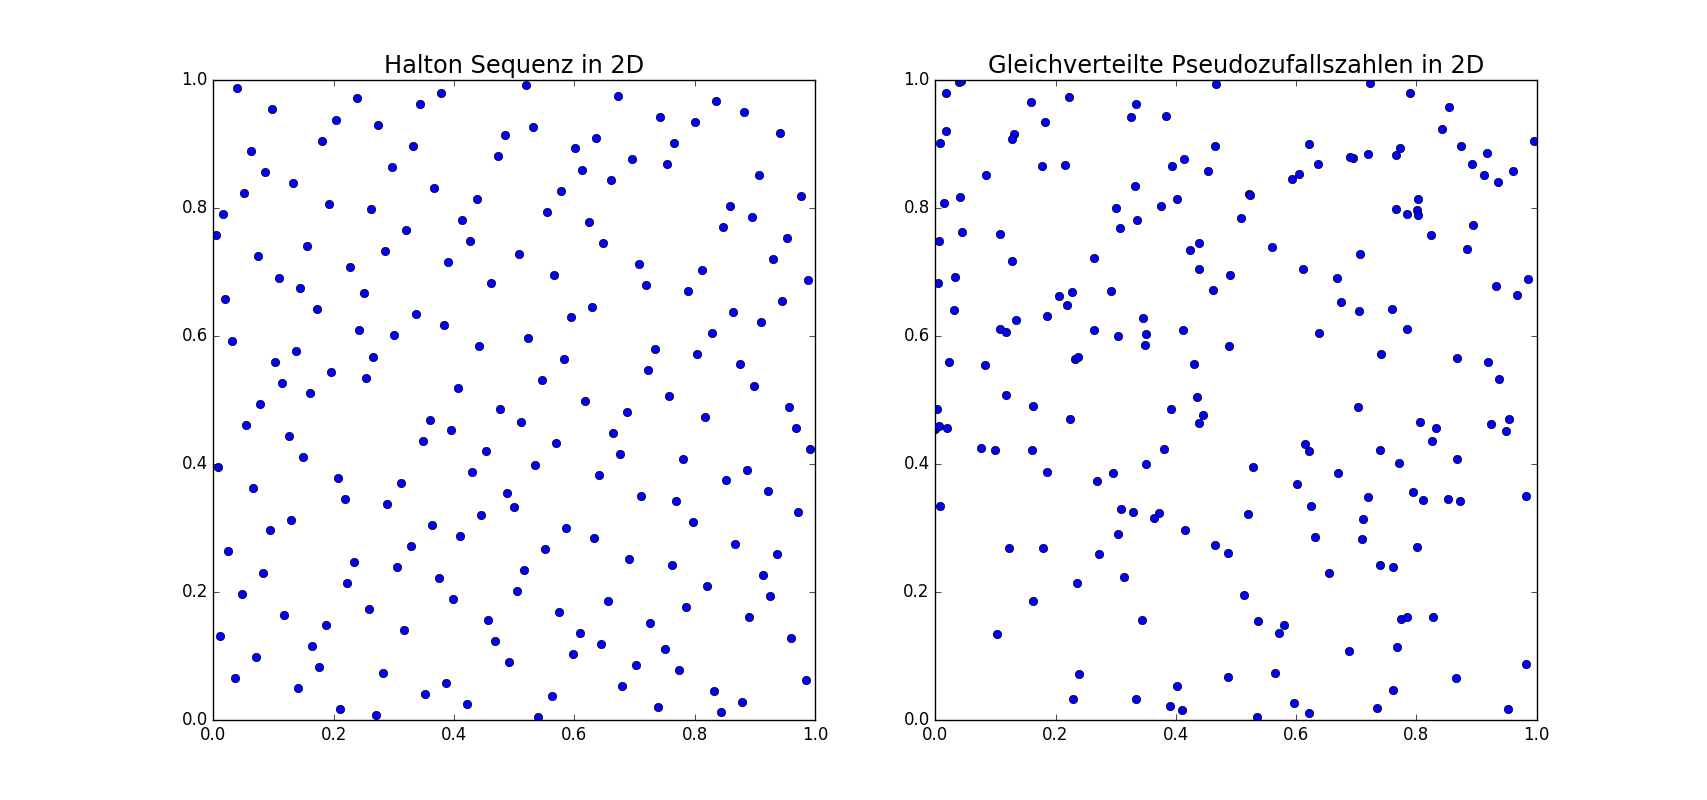
\includegraphics[width=\textwidth]{Figures/halton_numbers.png}
\caption{Darstellung der ersten 200 Halton Zahlen im zweidimensionalen und im Vergleich 200 gleichverteilte Pseudozufallszahlen. Die Halton Folge deckt die Fläche dabei viel gleichmäßiger ab.}
\label{fig:halton_numbers}
\end{figure}
Benötigt man wiederum Zufallszahlen mit einer anderen Verteilungsfunktion, so sind diese durch Anwendung der Inversionsmethode von Satz \ref{thinversionsmethode} erzeugbar.

\section{Approximation von Erwartungswert und Varianz}
Bevor wir den Kern der Schleife betrachten, wollen wir uns zuerst mit den eng miteinander zusammenhängenden Fragen \ref{mcsaveresults} und \ref{mcestimations} beschäftigen. Diese Fragen beziehen sich auf die Verwendung der einzelnen Zwischenergebnisse zur Approximation des Erwartungswertes und der Varianz und können wiederum vielseitig beantwortet werden.
\subsection*{Verarbeitung am Ende des Algorithmus}
Gegeben sei ein Zeitpunkt $T>0$ und die stochastische KGG (\ref{skgg}) zu einer Zufallsvariablen $Y$ und gesucht seien $\E[u(T,x,Y)]$ und $\text{var}(u(T,x,Y))$. Sind für $i=1,\dots,R$ die deterministischen Lösungen $u(T,x,y_i)$ gespeichert, so verwenden wir als Approximationen
\begin{align*}
\E[u(T,x,Y)]&\approx \frac{1}{R}\sum_{i=1}^R u(T,x,y_i)\eqqcolon m_R\\
\text{var}(u(T,x,Y)) &\approx \frac{1}{R-1}\sum_{i=1}^R(u(T,x,y_i)-m_R)^2.
\end{align*}
Wieso diese Approximationen sinnvoll sind, zeigt sich teilweise aus dem zentralen Grenzwertsatz \ref{thzentralgrenzwert}. Es folgt für unabhängige Stichproben $y_i$ die Aussage \[\sqrt{R}(m_R-\E[u(T,x,Y)])\xrightarrow{R\to\infty}\mathcal{N}(0,\text{var}(u(T,x,Y)))\]
und schlussendlich 
\[m_R=\E[u(T,x,Y)] + \mathcal{O}\left(\frac{1}{\sqrt{R}}\right).\]
In welchem Konvergenz-Sinne die letzte Aussage zu verstehen ist und welche Faktoren dabei in den letzten Term einfließen, sei an dieser Stelle nicht weiter ausgeführt. Wir werden diese Konvergenzordnung in Beispielen jedoch empirisch bestätigen.\\[0.2cm]
Die für die Approximation der Varianz verwendete Darstellung nennt man auch \emph{korrigierte Stichprobenvarianz}. Sie ist ein erwartungstreuer Schätzer der Varianz einer Stichprobe und ein Werkzeug aus der Statistik, welches wir hier nicht weiter erläutern werden.
\subsection*{Fortlaufende Berechnung}
Die Verarbeitung am Ende besitzt zwei große Nachteile:
\begin{itemize}
\item Sämtliche Zwischenergebnisse müssen gespeichert werden. Für die Mittelwertbildung alleine wäre dies zwar nicht nötig, jedoch für die Approximation der Varianz. An einer Beispielsrechnung soll der benötigte Arbeitsspeicher kurz verdeutlicht werden: Wird der eindimensionale Raum in 256 Punkten diskretisiert und benötigt jeder Punkt 8 Byte Speicher und führt man (durchaus realistisch) $R=100000$ Simulationen durch, so ergibt sich bereits ein Speicherbedarf von $\frac{256*100000*8\text{B}}{1024^2}\approx 200\text{MB}$. Dies ist also bereits für eine räumliche Dimension ein nicht unerheblicher Aufwand.
\item Die Methode zur Approximation der Varianz ist nicht stabil und stark anfällig für numerische Rechenfehler, insbesondere Überläufe (vgl. \autocite{cook08}). Aus diesem Grunde schlug Welford in \autocite{welford62} eine alternative Berechnungsmethode vor, welche wir im Folgenden erklären werden.
\end{itemize}
\begin{maththeorem}
\label{thiterativemk}
Für $x_1,\dots,x_k\in\R$ und $m_k=\frac{1}{k}\sum_{j=1}^kx_j$ gilt für $k\in\N$ die iterative Darstellung
\[m_k=m_{k-1}+\frac{x_k-m_{k-1}}{k},\quad \text{mit }\: m_0=0.\]
\end{maththeorem}
\begin{proof}
Wir zeigen mithilfe vollständiger Induktion die äquivalente Aussage, dass die Rekursion mit der Darstellung $m_k=\frac{1}{k}\sum_{j=1}^kx_j$ übereinstimmt.\\
I.A. ($k=1$): \[m_1=0+\frac{x_1-0}{1}=x_1=\sum_{j=1}^1x_j\quad\surd\]
I.S. ($k\leadsto k+1$):
\begin{align*}
m_{k+1}&\stackrel{Def}{=}m_k+\frac{x_{k+1}-m_k}{k+1}\\
&\stackrel{IV}{=}\frac{1}{k}\sum_{j=1}^kx_j+\frac{x_{k+1}}{k+1}-\frac{1}{k(k+1)}\sum_{j=1}^kx_j
\end{align*}
Multiplizieren wir nun mit $k(k+1)$ so erhalten wir
\begin{align*}
k(k+1)m_{k+1}&=(k+1)\sum_{j=1}^kx_j+kx_{k+1}-\sum_{j=1}^kx_j\\
&=k\sum_{j=1}^{k+1}x_j\\
\implies m_{k+1}&=\frac{1}{k+1}\sum_{j=1}^{k+1}x_j.
\end{align*}
\end{proof}
Wir haben nun eine iterative Methode zur Berechnung des Mittelwertes gewonnen, die nur den vorherigen Mittelwert, die neue Stichprobe und die Anzahl an Stichproben benötigt. Diese Methode ist robust gegen Überläufe und numerisch stabil. Viel wichtiger ist jedoch die iterative Berechnung des Varianzschätzers, welche auf ähnlichen Ideen basiert. Die Äquivalenz zur ursprünglichen Methode ist dabei allerdings schwieriger zu erkennen.
\begin{maththeorem}
Für $x_1,\dots,x_k\in\R$, $m_k$ wie in Satz \ref{thiterativemk} und $s_k=\sum_{j=1}^k(x_j-m_k)^2$ gilt für $k\in\N$ die iterative Darstellung
\[s_k=s_{k-1}+(x_k-m_k)(x_k-m_{k-1}),\quad\text{mit }s_0=0.\]
\end{maththeorem}
\begin{proof}
Es gilt für $j<k$ wegen $m_k=\frac{k-1}{k}m_{k-1}+\frac{1}{k}x_k$
\begin{align}
x_j-m_k&=x_j-m_{k-1}+\frac{1}{k}m_{k-1}-\frac{1}{k}x_k \nonumber\\
\label{eqn:mcvar1}
&=x_j-m_{k-1}-\frac{1}{k}(x_k-m_{k-1})\tag{*}\\
\label{eqn:mcvar2}
x_k-m_k&=\frac{k-1}{k}(x_k-m_{k-1}).\tag{**}
\end{align}
Dann gilt für $k\in\N$
\begin{align*}
s_k&=\sum_{j=1}^k(x_j-m_k)^2\stackrel{(\ref{eqn:mcvar2})}{=}\sum_{j=1}^{k-1}(x_j-m_k)^2+\frac{(k-1)^2}{k^2}(x_k-m_{k-1})^2\\
&\stackrel{(\ref{eqn:mcvar1})}{=}\sum_{j=1}^{k-1}(x_j-m_{k-1})^2-\frac{2}{k}(x_k-m_{k-1})\sum_{j=1}^{k-1}(x_j-m_{k-1})+\frac{k-1}{k^2}(x_k-m_{k-1})^2\\
&\quad +\frac{(k-1)^2}{k^2}(x_k-m_{k-1})^2\\
&=s_{k-1}-\frac{2}{k}(x_k-m_{k-1})\underbrace{\left((k-1)m_{k-1}-(k-1)m_{k-1}\right)}_{=0}+\underbrace{\frac{(k-1)^2+k-1}{k^2}}_{=\frac{k-1}{k}}(x_k-m_{k-1})^2\\
&=s_{k-1}+\frac{k-1}{k}(x_k-m_{k-1})\underbrace{(x_k-m_{k-1})}_{\stackrel{(\ref{eqn:mcvar2})}{=}\frac{k}{k-1}(x_k-m_k)}=s_{k-1}+(x_k-m_{k-1})(x_k-m_k).
\end{align*}
\end{proof}
Teilen wir nun $s_k$ noch durch $k-1$, so erhalten wir wieder die korrigierte Stichprobenvarianz. Wir benötigen dafür nur den vorherigen Wert $s_{k-1}$, die beiden letzten Mittelwerte, die neuste Stichprobe $x_k$ und die Stichprobenanzahl.
\section{Numerische Ergebnisse}
Man bemerkt schon an der Pseudocode-Darstellung der Monte-Carlo-Methode, dass der Bottleneck des Algorithmus in der Berechnung der Lösung der deterministischen KGG liegt. Der Zeitaufwand für alle anderen Operationen ist in Relation dazu vernachlässigbar klein. Ein großer Vorteil des Algorithmus ist seine \emph{embarrassingly parallel} Eigenschaft: Es ist kein nennenswerter Aufwand nötig, die Schleife zu parallelisieren und somit skaliert er perfekt mit der Anzahl an zur Verfügung stehenden Prozessoren. Dies ist eine erste Antwort auf Frage \ref{mcalgspeed}, jedoch sollte klar sein, dass das Lösen des deterministischen Systems dennoch so effizient wie möglich passieren muss. Ein Löser, der nur 0.1 Sekunden für ein einziges System benötigt und $R=100000$ Durchgänge erledigt, läuft ohne Parallelisierung bereits etwa 3 Stunden.\\
\subsection*{Konvergenz}
Anhand von Abbildung \ref{fig:mc_convergence_trial1} erkennen wir für Beispiel \ref{bsp:trial1} die (probabilistische) Konvergenz des Erwartungswertes und der Varianz mit ungefährer Ordnung $0.5$ für die Monte-Carlo-Methode. Diese Konvergenzordnung entspricht dem erwarteten stochastischen Fehler $\mathcal{O}\left(\dfrac{1}{R^{0.5}}\right)$, wobei $R$ die Anzahl an Realisierungen ist. Vergleichen wir dazu die Quasi-Monte-Carlo-Methode anhand desselben Beispiels in Abbildung \ref{fig:quasi_mc_convergence_trial1}, so erkennen wir eine bessere Konvergenzordnung und ein weniger chaotisches Verhalten des Fehlers.\\
Dennoch macht diese schlechte Konvergenzordnung das Verfahren sehr unattraktiv. Wir benötigen selbst für das simple Beispiel \ref{bsp:trial1} und die Quasi-Monte-Carlo-Methode bereits $R=100000$ Durchläufe für einen Fehler des Erwartungswertes in die Größenordnung $10^{-5}$.
\begin{figure}
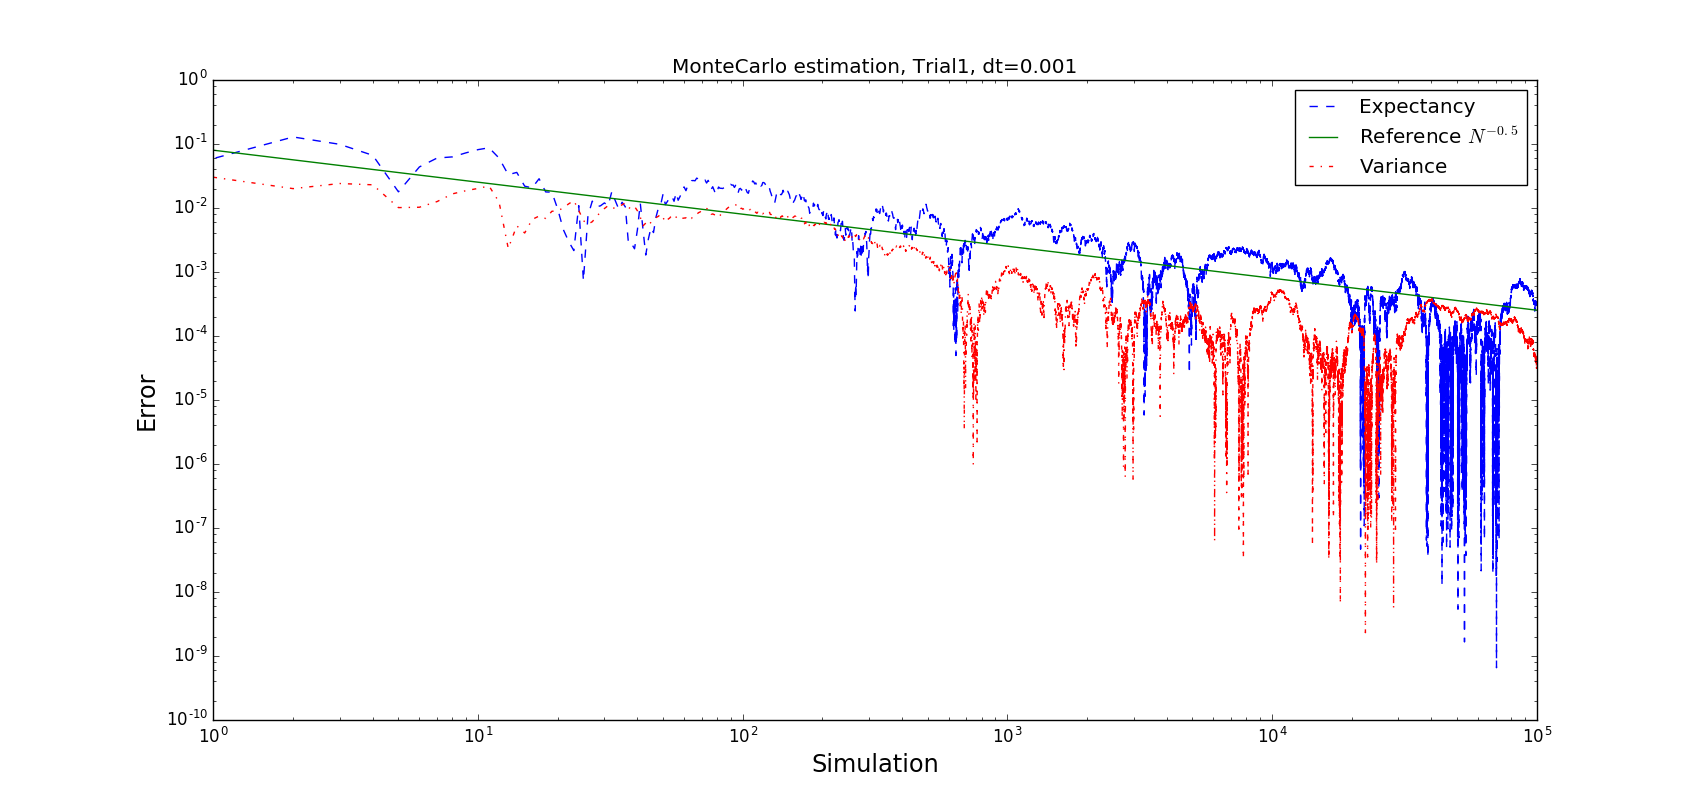
\includegraphics[width=\textwidth]{Figures/mc_convergence_trial1.png}
\caption{Konvergenz des Erwartungswertes und der Varianz von Beispiel \ref{bsp:trial1} mithilfe der Monte-Carlo-Methode zum Zeitpunkt $T=0.5$. Ordnungsplot mit Referenzlinie $0.08\frac{1}{\sqrt{R}}$ der erwarteten Ordnung.}
\label{fig:mc_convergence_trial1}
\end{figure}\\
\begin{figure}
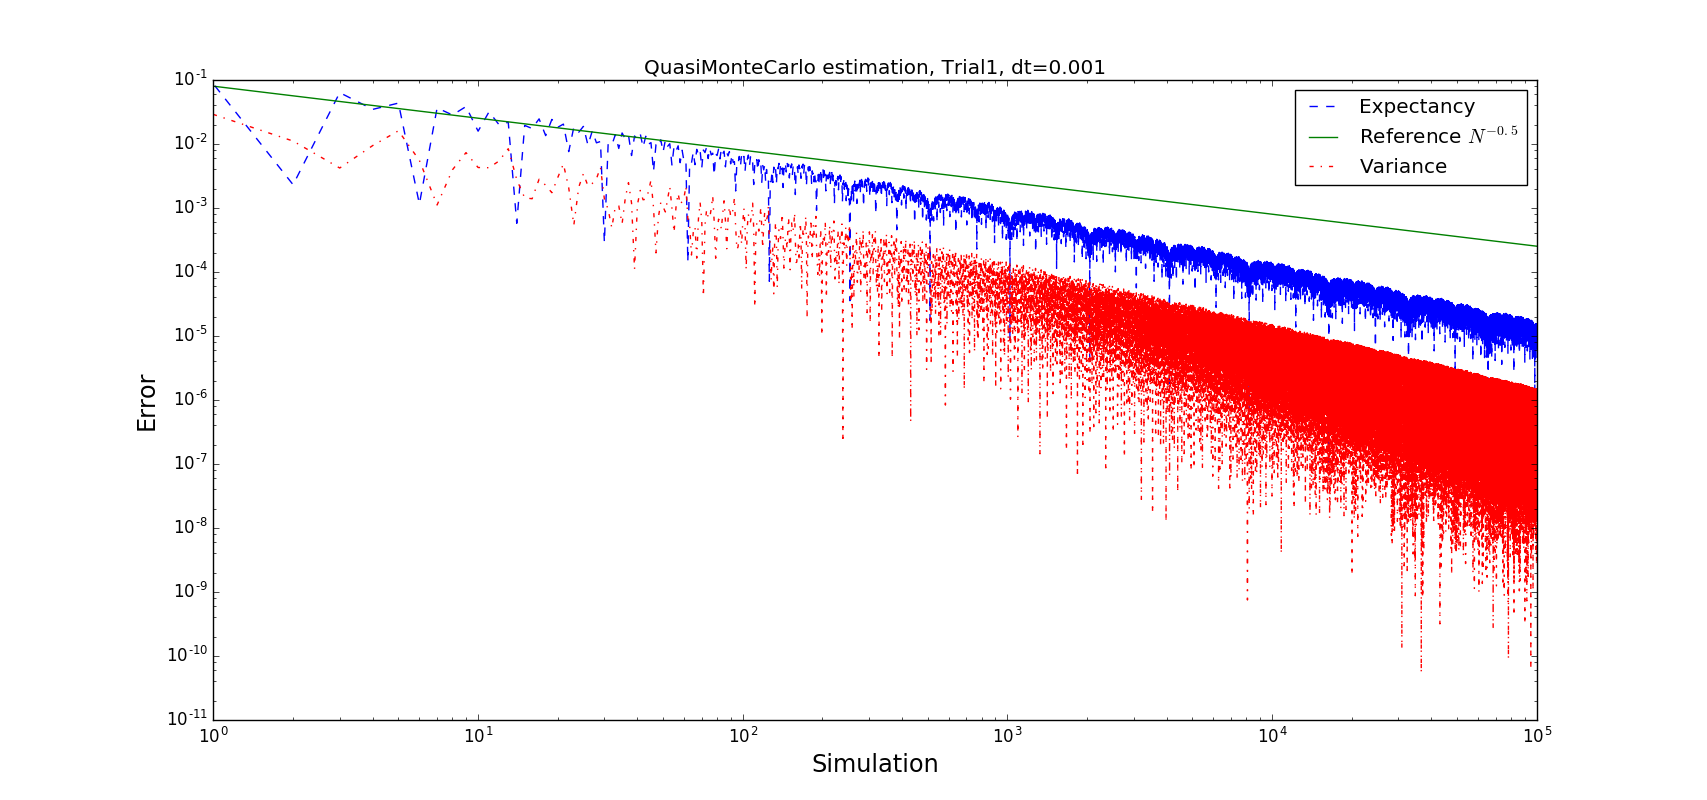
\includegraphics[width=\textwidth]{Figures/quasi_mc_convergence_trial1.png}
\caption{Konvergenz des Erwartungswertes und der Varianz von Beispiel \ref{bsp:trial1} mithilfe der Quasi-Monte-Carlo-Methode zum Zeitpunkt $T=0.5$. Ordnungsplot mit Referenzlinie $0.08\frac{1}{\sqrt{R}}$.}
Einen Vorteil allerdings bietet das Verfahren: Unabhängig von der Dimension des Zufallsraums erhalten wir jeweils dieselbe Konvergenzordnung und benötigen bis auf die Generierung der Komponenten von $Y$ keinen zeitlichen Mehraufwand für die Ausführung des Algorithmus im Vergleich zum eindimensionalen Fall. Diese Eigenschaft wird von keinem anderen Verfahren, die wir noch vorstellen werden, geteilt. Deren Rechenaufwand wird exponentiell mit der Größe des Zufallsvektors steigen. 
\label{fig:quasi_mc_convergence_trial1}
\end{figure}


